% Pure TikZ figure: no EPS conversion is needed.
\newcommand{\DoNotLoadEpstopdf}{}
\documentclass[tikz,border=0pt]{standalone}
\usepackage{amsmath,amssymb}
\usetikzlibrary{arrows.meta}
% Coordinates mirror the 1774 x 887 reference PNG; 1 unit = 0.1 mm.
\definecolor{pale}{RGB}{248,251,255}
\definecolor{edgeblue}{RGB}{145,189,247}
\definecolor{cost}{RGB}{191,48,47}
\definecolor{costbg}{RGB}{255,226,223}
\definecolor{cd}{RGB}{39,112,190}
\definecolor{cdbg}{RGB}{218,237,255}
\definecolor{mix}{RGB}{46,130,72}
\definecolor{mixbg}{RGB}{224,248,226}
\definecolor{purple}{RGB}{117,52,147}
\tikzset{
 every node/.style={inner sep=.6pt,scale=.62,font=\rmfamily\fontsize{6}{7}\selectfont},
 panel/.style={rounded corners=3pt,line width=.4pt},
 arrow/.style={-{Stealth[length=3mm,width=2.2mm]},draw=cd,line width=1pt},
}
\newcommand{\graphicon}[3]{%
 \begin{scope}[shift={(#1,#2)}]
 \coordinate (v1) at (0,-27); \coordinate (v2) at (22,-13);
 \coordinate (v3) at (25,13); \coordinate (v4) at (0,27);
 \coordinate (v5) at (-24,13); \coordinate (v6) at (-22,-13);
 \foreach \a/\b in {1/2,2/3,3/4,4/5,5/6,6/1,1/4,2/5,3/6}
   {\draw[#3,line width=.55pt] (v\a)--(v\b);}
 \foreach \k in {1,...,6}
   {\filldraw[fill=white,draw=#3,line width=.6pt] (v\k) circle (4.7);}
 \end{scope}}
% F01: six vertices and five edges, connected and acyclic.
\newcommand{\treeicon}[3]{%
 \begin{scope}[shift={(#1,#2)}]
 \coordinate (t1) at (0,-27); \coordinate (t2) at (-20,-5);
 \coordinate (t3) at (20,-5); \coordinate (t4) at (-30,25);
 \coordinate (t5) at (-8,25); \coordinate (t6) at (22,25);
 \foreach \a/\b in {1/2,1/3,2/4,2/5,3/6}
   {\draw[#3,line width=.55pt] (t\a)--(t\b);}
 \foreach \k in {1,...,6}
   {\filldraw[fill=white,draw=#3,line width=.6pt] (t\k) circle (4.7);}
 \end{scope}}
\newcommand{\layer}[2]{%
 \begin{scope}[shift={(#1,0)}]
 \node[font=\fontsize{7.3}{8}\selectfont] at (182,129) {Layer $l=#2$};
 \draw[panel,draw=cost!50,dashed,fill=costbg,fill opacity=.6] (0,147) rectangle (112,473);
 \draw[panel,draw=cd!45,dashed,fill=cdbg,fill opacity=.72] (122,147) rectangle (256,473);
 \draw[panel,draw=mix!45,dashed,fill=mixbg,fill opacity=.78] (263,147) rectangle (367,473);
 \node[font=\fontsize{6.8}{8}\selectfont] at (56,170) {$e^{-i\gamma_{#2}H_C}$};
 \node[font=\fontsize{6.8}{8}\selectfont] at (190,170) {$e^{-i\alpha_{#2}H_{CD}}$};
 \node[font=\fontsize{6.8}{8}\selectfont] at (315,170) {$e^{-i\beta_{#2}H_B}$};
 \draw[panel,draw=cost,line width=.7pt,fill=costbg] (12,204) rectangle (98,412);
 \node[align=center,font=\fontsize{7}{8}\selectfont] at (55,307) {$ZZ$\\cost\\unitary};
 \foreach \yy/\op in {224/YZ,269/ZY,349/YZ,394/ZY}{
  \draw[panel,draw=black,fill=white,line width=.55pt] (159,\yy-20) rectangle (220,\yy+20);
  \node[font=\fontsize{7}{8}\selectfont] at (190,\yy) {$\op$};
  \draw[panel,draw=black,fill=white,line width=.55pt] (291,\yy-20) rectangle (343,\yy+20);
  \node[font=\fontsize{7}{8}\selectfont] at (317,\yy) {$X$};
 }
 \node[align=center,font=\fontsize{5}{6}\selectfont] at (190,445) {Counterdiabatic\\driving unitary};
 \node[align=center,font=\fontsize{5}{6}\selectfont] at (315,445) {Mixing\\unitary};
 \end{scope}}
\begin{document}
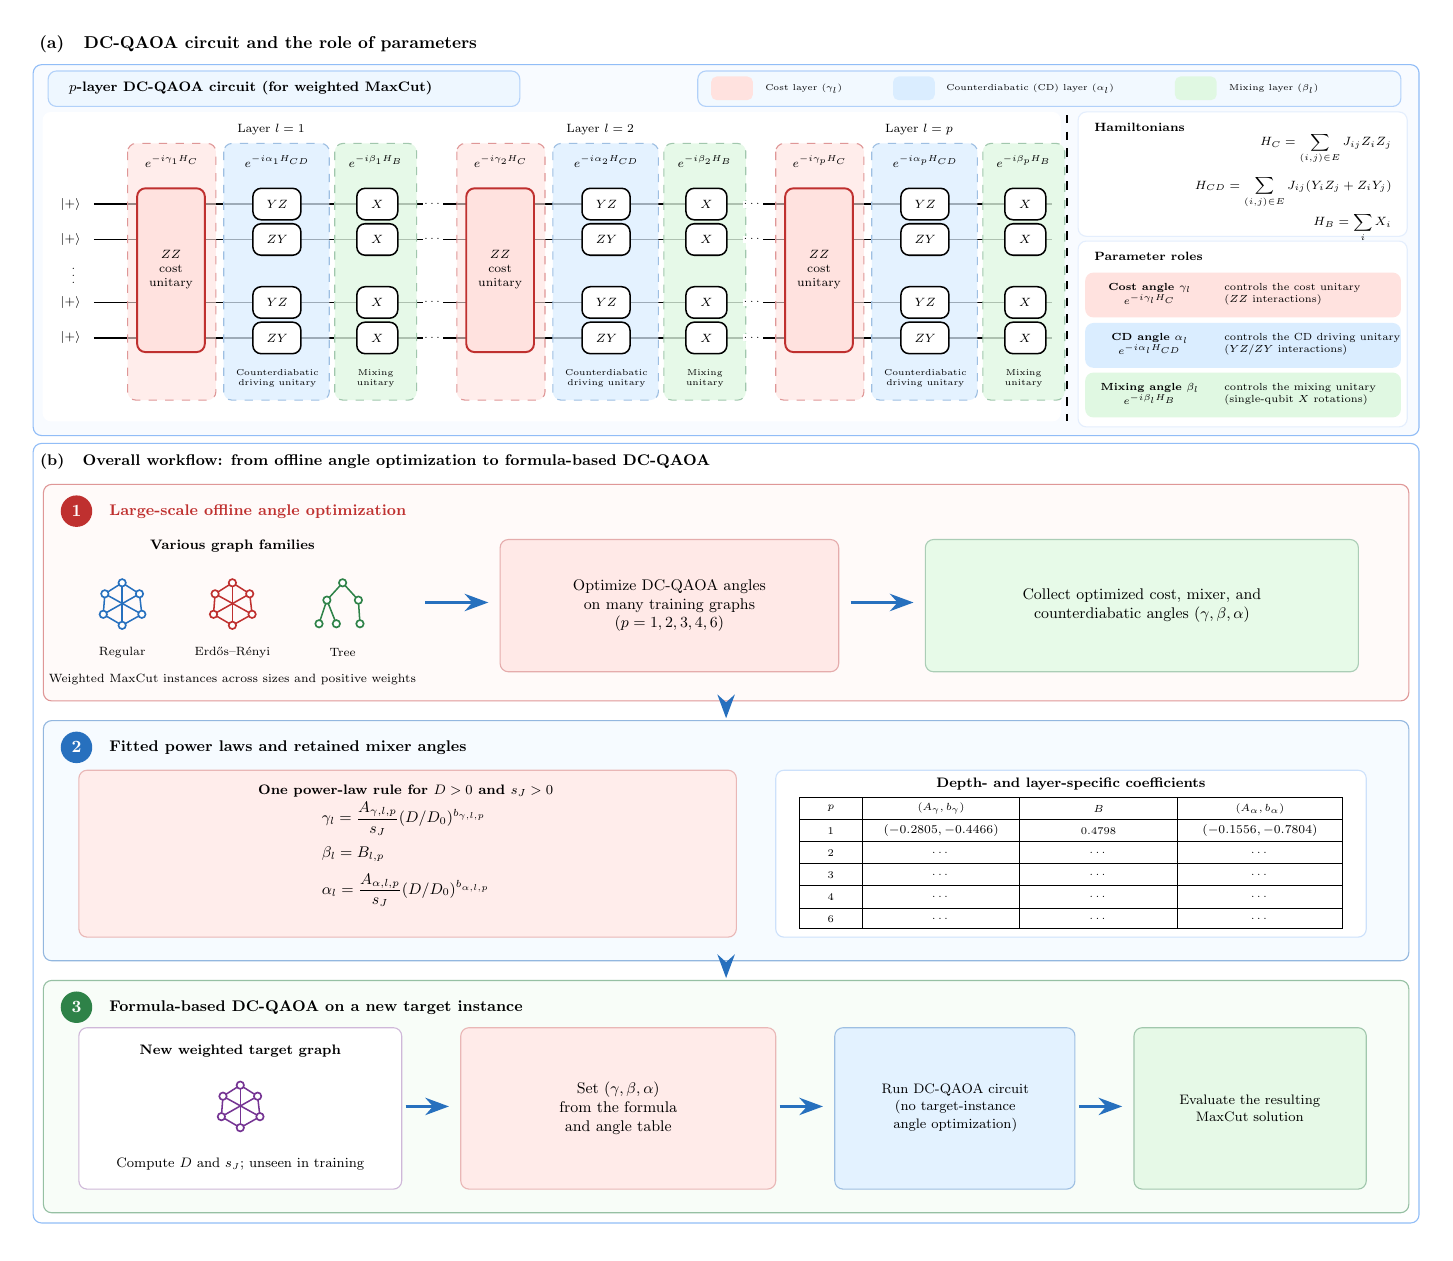
\begin{tikzpicture}[x=.1mm,y=-.1mm]
\useasboundingbox (0,0) rectangle (1774,1530);
\fill[white] (0,0) rectangle (1774,1530);
% Panel (a).
\node[anchor=west,font=\bfseries\fontsize{10.2}{11}\selectfont] at (13,21)
 {(a)\quad DC-QAOA circuit and the role of parameters};
\draw[panel,draw=edgeblue,fill=pale] (7,47) rectangle (1767,518);
\draw[panel,draw=edgeblue!70,fill=cdbg!45] (26,55) rectangle (625,100);
\node[anchor=west,font=\bfseries\fontsize{7.8}{8.5}\selectfont] at (51,77)
 {$p$-layer DC-QAOA circuit (for weighted MaxCut)};
\draw[panel,draw=edgeblue!70,fill=cdbg!35] (851,55) rectangle (1744,100);
\draw[fill=costbg,draw=none,rounded corners=2pt] (868,62) rectangle (921,92);
\node[anchor=west,font=\fontsize{5.3}{6}\selectfont] at (935,77) {Cost layer ($\gamma_l$)};
\draw[fill=cdbg,draw=none,rounded corners=2pt] (1099,62) rectangle (1152,92);
\node[anchor=west,font=\fontsize{5.3}{6}\selectfont] at (1165,77) {Counterdiabatic (CD) layer ($\alpha_l$)};
\draw[fill=mixbg,draw=none,rounded corners=2pt] (1457,62) rectangle (1510,92);
\node[anchor=west,font=\fontsize{5.3}{6}\selectfont] at (1524,77) {Mixing layer ($\beta_l$)};
\draw[panel,draw=none,fill=white] (19,107) rectangle (1312,500);
\draw[panel,draw=edgeblue!25,fill=white] (1334,107) rectangle (1752,265);
\draw[panel,draw=edgeblue!25,fill=white] (1334,271) rectangle (1752,507);
\draw[black,dashed,line width=.45pt] (1320,111)--(1320,500);
\foreach \yy in {224,269,349,394}{\draw[black,line width=.45pt] (84,\yy)--(1301,\yy);
 \node[anchor=east,font=\fontsize{7}{8}\selectfont] at (69,\yy) {$\lvert+\rangle$};}
\node at (58,309) {$\vdots$};
\layer{127}{1}\layer{545}{2}\layer{950}{p}
\foreach \xx in {515,921}{\foreach \yy in {224,269,349,394}
 {\node[fill=white] at (\xx,\yy) {$\cdots$};}}
\node[anchor=west,font=\bfseries\fontsize{7.4}{8}\selectfont] at (1353,127) {Hamiltonians};
\node[anchor=east,font=\fontsize{7}{8}\selectfont] at (1734,154)
 {$H_C=\displaystyle\sum_{(i,j)\in E}J_{ij}Z_iZ_j$};
\node[anchor=east,font=\fontsize{7}{8}\selectfont] at (1734,209)
 {$H_{CD}=\displaystyle\sum_{(i,j)\in E}J_{ij}(Y_iZ_j+Z_iY_j)$};
\node[anchor=east,font=\fontsize{7}{8}\selectfont] at (1734,254)
 {$H_B=\displaystyle\sum_iX_i$};
\node[anchor=west,font=\bfseries\fontsize{7.4}{8}\selectfont] at (1353,290) {Parameter roles};
\foreach \yy/\cc in {311/costbg,375/cdbg,438/mixbg}
 {\draw[panel,draw=none,fill=\cc] (1343,\yy) rectangle (1744,\yy+57);}
\node[align=center] at (1425,338) {\textbf{Cost angle $\gamma_l$}\\$e^{-i\gamma_lH_C}$};
\node[anchor=west,align=left] at (1518,338) {controls the cost unitary\\($ZZ$ interactions)};
\node[align=center] at (1425,402) {\textbf{CD angle $\alpha_l$}\\$e^{-i\alpha_lH_{CD}}$};
\node[anchor=west,align=left] at (1518,402) {controls the CD driving unitary\\($YZ/ZY$ interactions)};
\node[align=center] at (1425,465) {\textbf{Mixing angle $\beta_l$}\\$e^{-i\beta_lH_B}$};
\node[anchor=west,align=left] at (1518,465) {controls the mixing unitary\\(single-qubit $X$ rotations)};
% Panel (b): three full-width stages, read from top to bottom.
\draw[panel,draw=edgeblue,fill=white] (7,528) rectangle (1767,1518);
\node[anchor=west,font=\bfseries\fontsize{8.6}{9.5}\selectfont] at (14,551)
 {(b)\quad Overall workflow: from offline angle optimization to formula-based DC-QAOA};
\begin{scope}[every node/.append style={scale=1}]
% 1. Offline optimization.
\draw[panel,draw=cost!50,fill=costbg!18] (20,580) rectangle (1754,855);
\fill[cost] (62,614) circle (20);
\node[text=white,font=\bfseries\fontsize{10}{11}\selectfont] at (62,614) {1};
\node[anchor=west,text=cost,font=\bfseries\fontsize{9.5}{11}\selectfont] at (102,614)
 {Large-scale offline angle optimization};
\node[font=\bfseries\fontsize{8.2}{9.5}\selectfont] at (260,658) {Various graph families};
\graphicon{120}{732}{cd}\graphicon{260}{732}{cost}\treeicon{400}{732}{mix}
\node[font=\fontsize{7}{8}\selectfont] at (120,794) {Regular};
\node[font=\fontsize{7}{8}\selectfont] at (260,794) {Erd\H{o}s--R\'enyi};
\node[font=\fontsize{7}{8}\selectfont] at (400,794) {Tree};
\node[font=\fontsize{7.5}{9}\selectfont] at (260,828)
 {Weighted MaxCut instances across sizes and positive weights};
\draw[arrow] (505,730)--(585,730);
\draw[panel,draw=cost!40,fill=costbg!75] (600,650) rectangle (1030,818);
\node[align=center,font=\fontsize{9}{11}\selectfont] at (815,734)
 {Optimize DC-QAOA angles\\on many training graphs\\($p=1,2,3,4,6$)};
\draw[arrow] (1045,730)--(1125,730);
\draw[panel,draw=mix!40,fill=mixbg!78] (1140,650) rectangle (1690,818);
\node[align=center,font=\fontsize{9}{11}\selectfont] at (1415,734)
 {Collect optimized cost, mixer, and\\counterdiabatic angles $(\gamma,\beta,\alpha)$};
\draw[arrow] (887,857)--(887,877);
% 2. Offline prescription.
\draw[panel,draw=cd!50,fill=cdbg!24] (20,880) rectangle (1754,1185);
\fill[cd] (62,914) circle (20);
\node[text=white,font=\bfseries\fontsize{10}{11}\selectfont] at (62,914) {2};
\node[anchor=west,font=\bfseries\fontsize{9.5}{11}\selectfont] at (102,914)
 {Fitted power laws and retained mixer angles};
\draw[panel,draw=cost!35,fill=costbg!62] (65,943) rectangle (900,1155);
\node[font=\bfseries\fontsize{8.5}{10}\selectfont] at (480,969) {One power-law rule for $D>0$ and $s_J>0$};
\node[font=\fontsize{9}{11}\selectfont,align=left] at (480,1050)
 {$\gamma_l=\dfrac{A_{\gamma,l,p}}{s_J}(D/D_0)^{b_{\gamma,l,p}}$\\[6pt]
  $\beta_l=B_{l,p}$\\[6pt]
  $\alpha_l=\dfrac{A_{\alpha,l,p}}{s_J}(D/D_0)^{b_{\alpha,l,p}}$};
\draw[panel,draw=edgeblue!45,fill=white] (950,943) rectangle (1700,1155);
\node[font=\bfseries\fontsize{8.5}{10}\selectfont] at (1325,961) {Depth- and layer-specific coefficients};
\draw[line width=.45pt] (980,978) rectangle (1670,1144);
\foreach \xx in {1060,1260,1460}{\draw[line width=.35pt] (\xx,978)--(\xx,1144);}
\foreach \yy in {1006,1034,1062,1090,1118}{\draw[line width=.35pt] (980,\yy)--(1670,\yy);}
\node at (1020,992) {$p$};\node at (1160,992) {$(A_\gamma,b_\gamma)$};
\node at (1360,992) {$B$};\node at (1565,992) {$(A_\alpha,b_\alpha)$};
\node at (1020,1020) {1};\node[font=\fontsize{7}{8}\selectfont] at (1160,1020) {$(-0.2805,-0.4466)$};
\node at (1360,1020) {$0.4798$};\node[font=\fontsize{7}{8}\selectfont] at (1565,1020) {$(-0.1556,-0.7804)$};
\foreach \yy/\pp in {1048/2,1076/3,1104/4,1132/6}{
 \node at (1020,\yy) {\pp};
 \foreach \xx in {1160,1360,1565}{\node at (\xx,\yy) {$\cdots$};}}
\draw[arrow] (887,1187)--(887,1207);
% 3. Target-instance use, with no target-instance angle search.
\draw[panel,draw=mix!50,fill=mixbg!24] (20,1210) rectangle (1754,1505);
\fill[mix] (62,1244) circle (20);
\node[text=white,font=\bfseries\fontsize{10}{11}\selectfont] at (62,1244) {3};
\node[anchor=west,font=\bfseries\fontsize{9.5}{11}\selectfont] at (102,1244)
 {Formula-based DC-QAOA on a new target instance};
\draw[panel,draw=purple!35,fill=white] (65,1270) rectangle (475,1475);
\node[font=\bfseries\fontsize{8.5}{10}\selectfont] at (270,1300) {New weighted target graph};
\graphicon{270}{1370}{purple}
\node[font=\fontsize{7.7}{9}\selectfont] at (270,1443) {Compute $D$ and $s_J$; unseen in training};
\draw[arrow] (480,1370)--(535,1370);
\draw[panel,draw=cost!35,fill=costbg!68] (550,1270) rectangle (950,1475);
\node[align=center,font=\fontsize{9}{11}\selectfont] at (750,1372)
 {Set $(\gamma,\beta,\alpha)$\\from the formula\\and angle table};
\draw[arrow] (955,1370)--(1010,1370);
\draw[panel,draw=cd!45,fill=cdbg!75] (1025,1270) rectangle (1330,1475);
\node[align=center,font=\fontsize{8.5}{10}\selectfont] at (1178,1372)
 {Run DC-QAOA circuit\\(no target-instance\\angle optimization)};
\draw[arrow] (1335,1370)--(1390,1370);
\draw[panel,draw=mix!45,fill=mixbg!82] (1405,1270) rectangle (1700,1475);
\node[align=center,font=\fontsize{8.5}{10}\selectfont] at (1552,1372)
 {Evaluate the resulting\\MaxCut solution};
\end{scope}
\end{tikzpicture}
\end{document}
